\documentclass[aspectratio=169,11pt]{beamer}
\usepackage{beamerucad}
\usepackage{listings}
\definecolor{ckw}{HTML}{2563AB}\definecolor{cst}{HTML}{2E8B57}\definecolor{ccm}{HTML}{8A8F98}
\lstdefinestyle{py}{language=Python,basicstyle=\ttfamily\footnotesize,
 keywordstyle=\color{ckw}\bfseries,stringstyle=\color{cst},commentstyle=\color{ccm}\itshape,
 showstringspaces=false,columns=fullflexible,keepspaces=true,
 backgroundcolor=\color{ucadband!8},frame=leftline,framerule=2.5pt,rulecolor=\color{ucadband},
 xleftmargin=8pt,aboveskip=3pt,belowskip=1pt,basewidth=0.5em}
\lstset{style=py}
\title{Introduction au ML — Séance 7}
\subtitle{Valider et régler sans tricher : la validation croisée}
\author{Dr. El Hadji Bassirou TOURÉ}
\institute{Département de Mathématiques et Informatique\\ Faculté des Sciences et Techniques\\ Université Cheikh Anta Diop de Dakar}
\date{}
\setucadfoot{Introduction au ML --- Séance 7 \quad\textbullet\quad Dr. El Hadji Bassirou TOURÉ --- DMI/FST/UCAD}
\graphicspath{{figs/}}
\begin{document}

\begin{frame}[plain,noframenumbering]\titlepage\end{frame}

\begin{frame}{Objectifs de la séance}
\begin{ucaddef}[Contenu]
{\small La Séance 6 a laissé deux curseurs en suspens — le seuil et \texttt{C} — avec une interdiction : ne pas les régler sur le test. Cette séance construit le protocole qui permet de régler \emph{tous} les réglages du cours sans se mentir.}
\end{ucaddef}
\begin{itemize}\small
  \item Les \textbf{trois usages} des données : entraîner, régler, juger — et pourquoi ils ne se mélangent pas.
  \item La \textbf{variance du découpage} : pourquoi un score sur un seul split ne prouve presque rien.
  \item La \textbf{validation croisée} ($k$ plis), construite à la main puis vérifiée contre \texttt{cross\_val\_score}.
  \item Régler un hyperparamètre : la \textbf{courbe de validation} ($\alpha$ de Ridge, profondeur d'arbre).
  \item Plusieurs réglages à la fois : \textbf{GridSearchCV}, sa double boucle et son coût.
  \item Le \textbf{seuil} de la Séance 6 enfin réglé proprement, par \texttt{cross\_val\_predict}.
\end{itemize}
\end{frame}

% #####################################################################
\section{Trois usages, un seul jeu de données}

\begin{frame}{Là où la Séance 6 s'est arrêtée}
\begin{ucadfront}[Le constat du mini-défi]
{\small Régler le seuil \emph{en regardant le test} donnait un chiffre flatteur mais sans valeur — la fuite de la Séance 4, version hyperparamètre. La réparation proposée — réserver une tranche de \textbf{validation} — a soulevé deux objections immédiates : elle \textbf{ampute l'entraînement}, et son verdict \textbf{dépend du hasard du découpage}. La séance résout les deux.}
\end{ucadfront}
{\small L'inventaire des réglages accumulés depuis le début du cours : la profondeur de l'arbre (S3), le $k$ du $k$-NN (S4), l'$\alpha$ de Ridge (S5), le \texttt{C} et le seuil de la logistique (S6). Tous attendent le même protocole.}
\end{frame}

\begin{frame}{Paramètres et hyperparamètres : deux familles de réglages}
\begin{ucaddef}[Définition]
{\small Les \textbf{paramètres} ($b$, $\mathbf{w}$, les seuils de coupure d'un arbre...) sont appris \emph{par} l'entraînement. Les \textbf{hyperparamètres} (profondeur, $k$, $\alpha$, \texttt{C}, seuil de décision...) sont choisis \emph{avant} ou \emph{autour} de l'entraînement — l'algorithme ne peut pas les apprendre lui-même.}
\end{ucaddef}
{\small Le test du « qui choisit ? » : si \texttt{fit} le calcule, c'est un paramètre ; si c'est un argument du constructeur (ou un curseur appliqué après), c'est un hyperparamètre. Or un hyperparamètre mal choisi peut ruiner le meilleur des algorithmes — la profondeur $12$ de l'arbre en S5 divisait son $R^2$ par deux. Il faut donc des données pour les \emph{départager}.}
\end{frame}

\begin{frame}{L'idée : trois usages, trois jeux}
\begin{ucadfront}[Analogie]
{\small La préparation au baccalauréat : les \textbf{annales} pour apprendre (entraînement), le \textbf{bac blanc} pour choisir sa stratégie (réglage), le \textbf{vrai bac} pour juger — une seule fois. Réviser sur les sujets du vrai bac, c'est falsifier la mesure.}
\end{ucadfront}
\begin{ucaddef}[L'idée en une phrase]
{\small Toute donnée qui a servi à \textbf{choisir} quelque chose — un poids, un hyperparamètre, un seuil — ne peut plus servir à \textbf{juger} le résultat de ce choix.}
\end{ucaddef}
\centering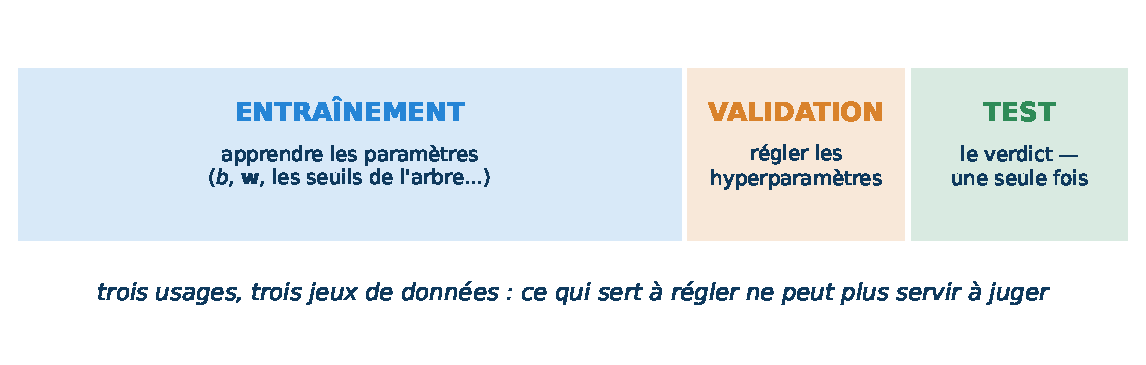
\includegraphics[width=0.58\linewidth]{f7_trois_usages}
\end{frame}

\begin{frame}{Le test ne sert qu'une fois}
\begin{ucadpiege}[Le bac blanc repassé cinquante fois]
{\small Évaluer cinquante variantes sur le test et garder la meilleure, c'est faire du test un jeu de réglage : le chiffre final est \emph{optimiste par construction} — la variante gagnante a en partie gagné par chance, et cette chance ne se reproduira pas en production. Le test se consulte \textbf{une seule fois}, à la toute fin, quand tous les choix sont gelés.}
\end{ucadpiege}
{\small D'où la question pratique de toute la séance : avec un budget de données fini, comment fabriquer un \emph{juge de réglage} fiable sans sacrifier ni l'entraînement, ni le test ?}
\end{frame}

% #####################################################################
\section{La variance du découpage}

\begin{frame}{Exemple — la même recette, cinq découpages}
\begin{ucadex}[La logistique du paludisme, cinq splits différents]
{\small La même recette exactement — Pipeline standardisation $+$ logistique — entraînée et évaluée sur cinq découpages train/test (mêmes proportions, graines différentes) :
\begin{center}\renewcommand{\arraystretch}{1.05}\begin{tabular}{c|ccccc}
découpage & $0$ & $1$ & $2$ & $3$ & $4$\\\hline
AUC & $0{,}691$ & $0{,}702$ & $0{,}688$ & $0{,}704$ & $0{,}692$\\
\end{tabular}\end{center}
Moyenne $0{,}6955$, écart-type $0{,}0064$, \textbf{étendue $0{,}016$}. Rien n'a changé dans la recette — seul le hasard du découpage a parlé.}
\end{ucadex}
\end{frame}

\begin{frame}{Ce que cette variance interdit de conclure}
\centering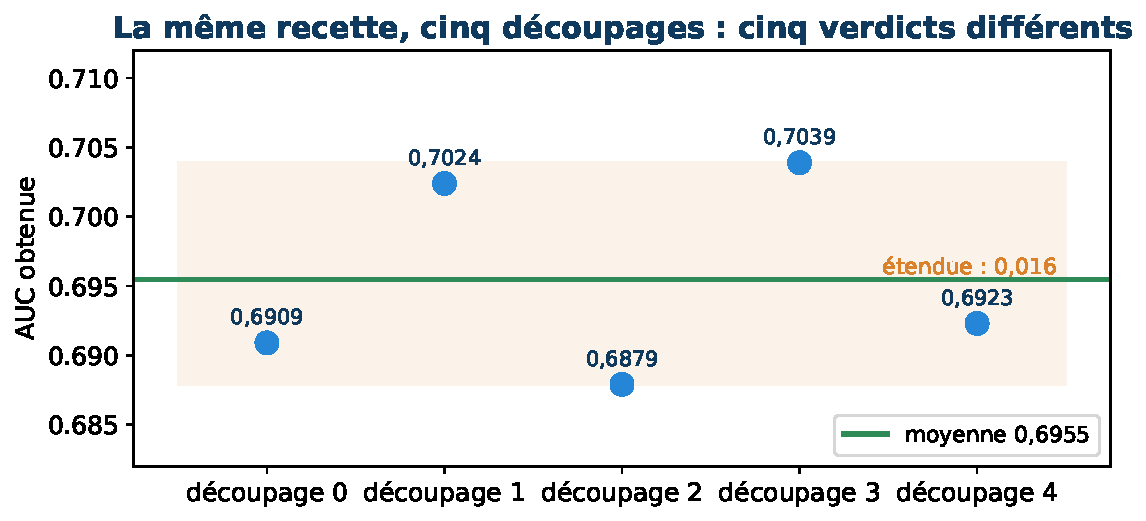
\includegraphics[width=0.62\linewidth]{f7_variance}
\vspace{-2pt}

{\small Un score d'évaluation n'est pas \emph{le} niveau du modèle : c'est une \textbf{mesure bruitée} de ce niveau, dont le bruit vient du découpage. Comparer deux recettes qui diffèrent de $0{,}01$ sur \emph{un seul} split, c'est comparer deux mesures dont le bruit propre vaut déjà $0{,}016$ : le classement peut s'inverser au prochain tirage.}
\end{frame}

\begin{frame}{Exercice — peut-on conclure ?}
\begin{ucadrec}[Énoncé]
{\small Sur un unique découpage, la recette A obtient une AUC de $0{,}72$ et la recette B une AUC de $0{,}73$. Au vu de l'étendue mesurée ci-dessus ($0{,}016$ entre découpages), peut-on déclarer B meilleure que A ? Que faudrait-il pour trancher ?}
\end{ucadrec}
\pause
\begin{ucadex}[Correction]
{\small Non : l'écart observé ($0{,}01$) est \emph{inférieur} au bruit typique du découpage ($0{,}016$) — l'ordre pourrait s'inverser sur un autre split. Pour trancher, il faut \textbf{plusieurs} évaluations de chaque recette (plusieurs découpages) et comparer les \emph{moyennes} en regard des écarts-types. C'est exactement ce que la validation croisée va industrialiser.}
\end{ucadex}
\end{frame}

% #####################################################################
\section{La validation croisée}

\begin{frame}{L'idée : chacun son tour d'être le juge}
\begin{ucadfront}[Analogie]
{\small Une tontine : chaque membre cotise à tous les tours, et reçoit la cagnotte \emph{une fois}, à son tour. La validation croisée organise les données pareil : chaque pli sert à entraîner à tous les tours, sauf au sien — où il devient le juge. À la fin, \emph{toutes} les données ont entraîné, \emph{toutes} ont jugé, et aucune n'a fait les deux en même temps.}
\end{ucadfront}
\begin{ucaddef}[L'idée en une phrase]
{\small La \textbf{validation croisée} à $k$ plis découpe l'entraînement en $k$ morceaux, fait $k$ entraînements (à chaque tour, un pli différent joue la validation), et rend la \textbf{moyenne} des $k$ scores — avec son écart-type, qui mesure le bruit.}
\end{ucaddef}
\end{frame}

\begin{frame}{La validation croisée, formellement}
\begin{ucaddef}[Définition]
{\small Soit l'entraînement partitionné en $k$ plis $V_1, \dots, V_k$ de tailles égales. Pour chaque tour $j$, la recette est entraînée sur tout sauf $V_j$, puis notée sur $V_j$ : score$_j$. Le verdict est la moyenne, l'incertitude est l'écart-type.}
\end{ucaddef}
\ucadformula{\text{CV}_k \;=\; \frac{1}{k}\sum_{j=1}^{k} \text{score}_j \qquad\qquad s \;=\; \sqrt{\tfrac{1}{k}\textstyle\sum_j (\text{score}_j - \text{CV}_k)^2}}
{\small Chaque observation est jugée \emph{exactement une fois}, par un modèle qui ne l'a jamais vue — c'est la propriété centrale. Le prix : $k$ entraînements au lieu d'un. Et le test, lui, reste intact dans son coffre.}
\end{frame}

\begin{frame}{Le schéma des cinq plis}
\centering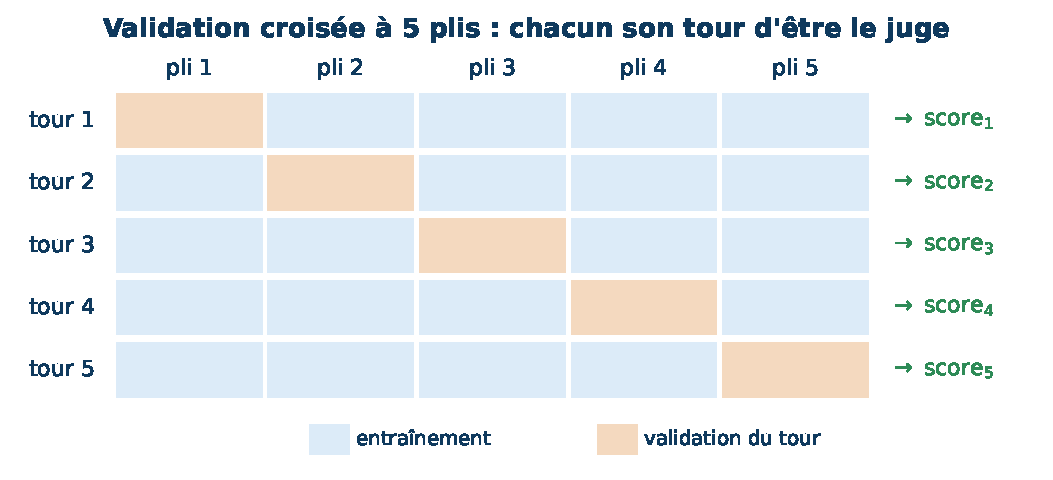
\includegraphics[width=0.74\linewidth]{f7_kfold}
\vspace{-2pt}

{\small À chaque tour (ligne), le pli orange juge, les plis bleus entraînent. Cinq tours, cinq scores, une moyenne — et chaque donnée n'a été juge qu'une fois, jamais de sa propre recette.}
\end{frame}

\begin{frame}{Le mécanisme — la CV à la main (1/2)}
\begin{ucadex}[Six points, trois plis, trois équations normales]
{\small Le jeu jouet : $x = (1,2,3,4,5,6)$, $y = (2,2,4,5,5,7)$, découpé en trois plis consécutifs $\{1,2\}$, $\{3,4\}$, $\{5,6\}$. À chaque tour, la droite est ajustée par les \textbf{formules fermées de la Séance 5} sur les quatre points restants :
\begin{center}\footnotesize\renewcommand{\arraystretch}{1.12}\begin{tabular}{c|c|c|c|c}
tour & valide sur & entraîne sur & droite apprise & MSE de validation\\\hline
$1$ & $\{1,2\}$ & $\{3,4,5,6\}$ & $b=1{,}2$, $w=0{,}9$ & $0{,}505$\\
$2$ & $\{3,4\}$ & $\{1,2,5,6\}$ & $b=0{,}5$, $w=1{,}0$ & $0{,}250$\\
$3$ & $\{5,6\}$ & $\{1,2,3,4\}$ & $b=0{,}5$, $w=1{,}1$ & $0{,}505$\\
\end{tabular}\end{center}
Le tour $3$ entraîne sur $\{1,2,3,4\}$ — et retrouve \textbf{exactement} le $b = 0{,}5$, $w = 1{,}1$ du jouet de la Séance 5 : même données, même équation normale, même droite.}
\end{ucadex}
\end{frame}

\begin{frame}{Le mécanisme — la CV à la main (2/2)}
\centering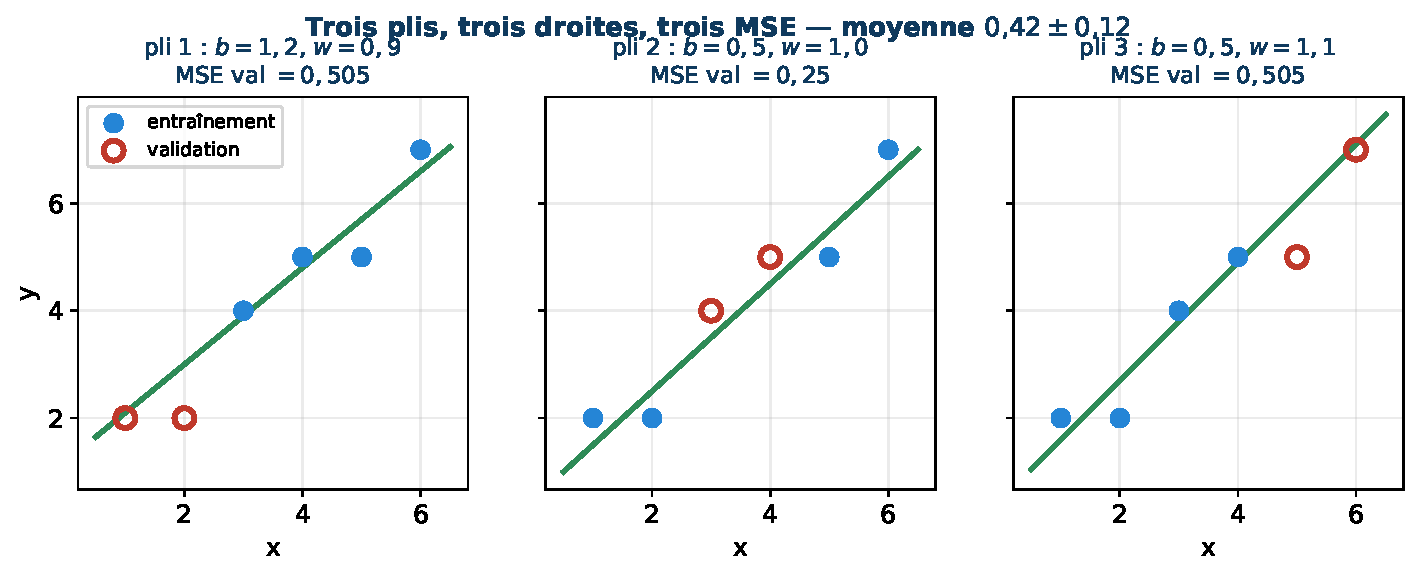
\includegraphics[width=0.84\linewidth]{f7_toy_folds}
\vspace{-2pt}

{\small Trois droites différentes — chaque tour apprend sur des données différentes — et trois MSE de validation. Le verdict : $\text{CV}_3 = (0{,}505 + 0{,}250 + 0{,}505)/3 = \mathbf{0{,}42}$, écart-type $\mathbf{0{,}12}$. \texttt{cross\_val\_score} rend exactement $(0{,}505;\ 0{,}250;\ 0{,}505)$ : le mécanisme est celui-là, rien de plus.}
\end{frame}

\begin{frame}{Ce que la CV ne fabrique pas}
\begin{ucadpiege}[Trois droites, mais lesquelles garder ?]
{\small Aucune : la validation croisée n'élit pas un des $k$ modèles — elle évalue une \textbf{recette} (un algorithme et ses hyperparamètres). Une fois la recette validée, le modèle final est \textbf{réentraîné sur tout l'entraînement} : il profite alors de toutes les données, et la CV a déjà dit ce qu'il vaudra, en moyenne.}
\end{ucadpiege}
{\small Distinguer trois objets : la \emph{recette} (ce que la CV note), les $k$ \emph{modèles intermédiaires} (jetables, ils n'existent que pour noter), et le \emph{modèle final} (réentraîné sur tout, c'est lui qui part en production).}
\end{frame}

\begin{frame}{La stratification : la classe rare dans chaque pli}
\begin{ucaddef}[L'idée en une phrase]
{\small Sur une cible rare ($11{,}8\,\%$ de paludisme), un pli tiré au hasard peut être anormalement pauvre ou riche en positifs — son verdict est faussé. \textbf{StratifiedKFold} impose à chaque pli la proportion globale, comme le split stratifié de la Séance 6.}
\end{ucaddef}
\begin{ucadex}[Parts de positifs par pli sur l'entraînement du paludisme]
{\small \begin{center}\footnotesize\renewcommand{\arraystretch}{1.05}\begin{tabular}{l|ccccc}
\texttt{KFold} & $0{,}106$ & $0{,}128$ & $0{,}124$ & $0{,}108$ & $0{,}123$\\
\texttt{StratifiedKFold} & $0{,}1175$ & $0{,}1175$ & $0{,}1175$ & $0{,}1175$ & $0{,}1181$\\
\end{tabular}\end{center}
Sans stratification, le pli le plus pauvre ($10{,}6\,\%$) et le plus riche ($12{,}8\,\%$) jugent des situations sensiblement différentes. Règle : \textbf{classification $\Rightarrow$ plis stratifiés}, toujours.}
\end{ucadex}
\end{frame}

\begin{frame}{Combien de plis ?}
{\small Le choix de $k$ est un compromis coût/fiabilité :}
\begin{itemize}\small
  \item $k = 5$ : le standard — chaque tour entraîne sur $80\,\%$ des données, cinq entraînements seulement ;
  \item $k = 10$ : verdict un peu plus stable, deux fois plus cher — courant quand les données sont rares ;
  \item $k = n$ (\emph{leave-one-out}) : chaque point jugé par un modèle entraîné sur tous les autres — $n$ entraînements, réservé aux très petits jeux ;
  \item $k = 2$ ou $3$ : rapide, mais chaque tour n'entraîne que sur la moitié ou les deux tiers — le verdict sous-estime la recette.
\end{itemize}
{\small Dans tout le cours : \textbf{$k = 5$, stratifié en classification}, sauf mention contraire.}
\end{frame}

\begin{frame}[fragile]{En pratique : cross\_val\_score}
\begin{lstlisting}
from sklearn.model_selection import cross_val_score, StratifiedKFold

pipe = make_pipeline(StandardScaler(),
                     LogisticRegression(max_iter=1000, random_state=0))
cv = StratifiedKFold(n_splits=5, shuffle=True, random_state=0)
scores = cross_val_score(pipe, X_train, y_train, cv=cv, scoring="roc_auc")
print(scores.mean(), "+/-", scores.std())
\end{lstlisting}
{\small Trois détails qui comptent : la recette passée est le \textbf{Pipeline entier} (la standardisation est refaite \emph{dans} chaque pli — la raison arrive dans les pièges) ; \texttt{scoring} nomme la métrique de la Séance 6 (\texttt{"roc\_auc"}, \texttt{"recall"}, ...) ; et seul \texttt{X\_train} entre — le test n'approche jamais la CV.}
\end{frame}

\begin{frame}{Exercice — dépouiller une validation croisée}
\begin{ucadrec}[Énoncé]
{\small Une CV à $5$ plis rend les scores $(0{,}70;\ 0{,}74;\ 0{,}68;\ 0{,}73;\ 0{,}70)$ pour la recette A, et un \emph{unique} split rend $0{,}75$ pour la recette B. Calculer la moyenne de A (les cinq valeurs somment à $3{,}55$), puis dire laquelle des deux affirmations est la plus solide : « A vaut environ $0{,}71$ » ou « B vaut $0{,}75$ ».}
\end{ucadrec}
\pause
\begin{ucadex}[Correction]
{\small Moyenne de A : $3{,}55/5 = \mathbf{0{,}71}$, avec une dispersion visible d'environ $\pm 0{,}02$. L'affirmation solide est celle sur A : cinq mesures indépendantes encadrent le niveau. Le $0{,}75$ de B est \emph{une seule} mesure bruitée — au vu d'un bruit typique de $\pm 0{,}02$, B pourrait valoir $0{,}71$ comme $0{,}77$. Conclure « B bat A » serait prématuré : il faut la CV de B.}
\end{ucadex}
\end{frame}

% #####################################################################
\section{Régler un hyperparamètre}

\begin{frame}{L'idée : une note de CV par valeur du curseur}
\begin{ucaddef}[L'idée en une phrase]
{\small Pour régler un hyperparamètre, il suffit de donner à \emph{chaque valeur candidate} sa note de validation croisée, puis de garder la valeur la mieux notée — le test n'a pas été consulté, le réglage est honnête.}
\end{ucaddef}
{\small Le tracé de la note CV en fonction de la valeur s'appelle la \textbf{courbe de validation}. Sa forme typique est déjà connue : c'est la courbe en U de la Séance 5 (sous-ajustement d'un côté, sur-ajustement de l'autre) — mais mesurée proprement, par CV, au lieu d'un unique split.}
\end{frame}

\begin{frame}{Exemple — l'$\alpha$ de Ridge, version honnête}
\begin{ucadex}[La sinusoïde de la Séance 5, refaite au propre]
{\small En Séance 5, l'$\alpha$ du polynôme de degré $15$ avait été choisi \emph{en regardant} les $20$ points de validation — un réglage sur split unique. Reprise : CV à $5$ plis \textbf{sur les $30$ points d'entraînement seulement} :
\begin{center}\footnotesize\renewcommand{\arraystretch}{1.05}\begin{tabular}{c|ccccccc}
$\alpha$ & $10^{-4}$ & $10^{-3}$ & $10^{-2}$ & $\mathbf{0{,}1}$ & $1$ & $10$ & $100$\\\hline
RMSE CV & $1{,}33$ & $0{,}69$ & $0{,}67$ & $\mathbf{0{,}42}$ & $0{,}69$ & $0{,}49$ & $0{,}84$\\
\end{tabular}\end{center}
Meilleur : $\alpha = 0{,}1$. Verdict final sur les $20$ points jamais touchés : RMSE $= 0{,}336$ — la CV retrouve le bon réglage \emph{sans avoir eu besoin de tricher}.}
\end{ucadex}
\end{frame}

\begin{frame}{La courbe de validation de Ridge}
\centering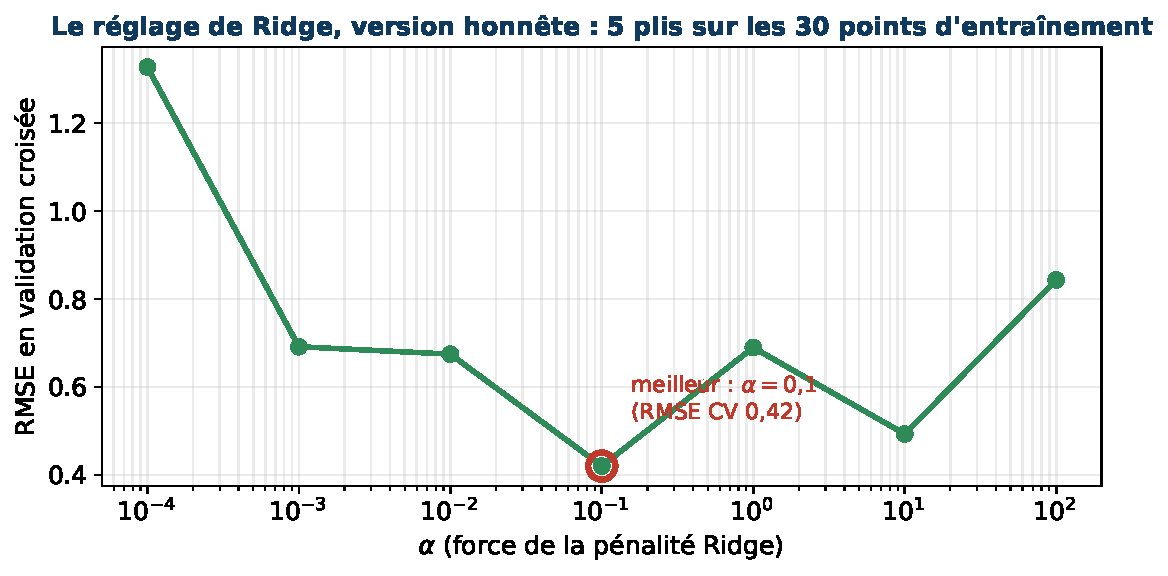
\includegraphics[width=0.62\linewidth]{f7_ridge_cv}
\vspace{-2pt}

{\small La forme générale est le U attendu — trop peu de pénalité : l'explosion du degré $15$ ; trop : le sous-ajustement. Le creux local à $\alpha = 1$ rappelle une leçon de la section précédente : avec $30$ points seulement, la CV reste une mesure \emph{bruitée} — la tendance se lit, les petites bosses ne se surinterprètent pas.}
\end{frame}

\begin{frame}{Exemple — la profondeur d'arbre, vue d'avance}
\centering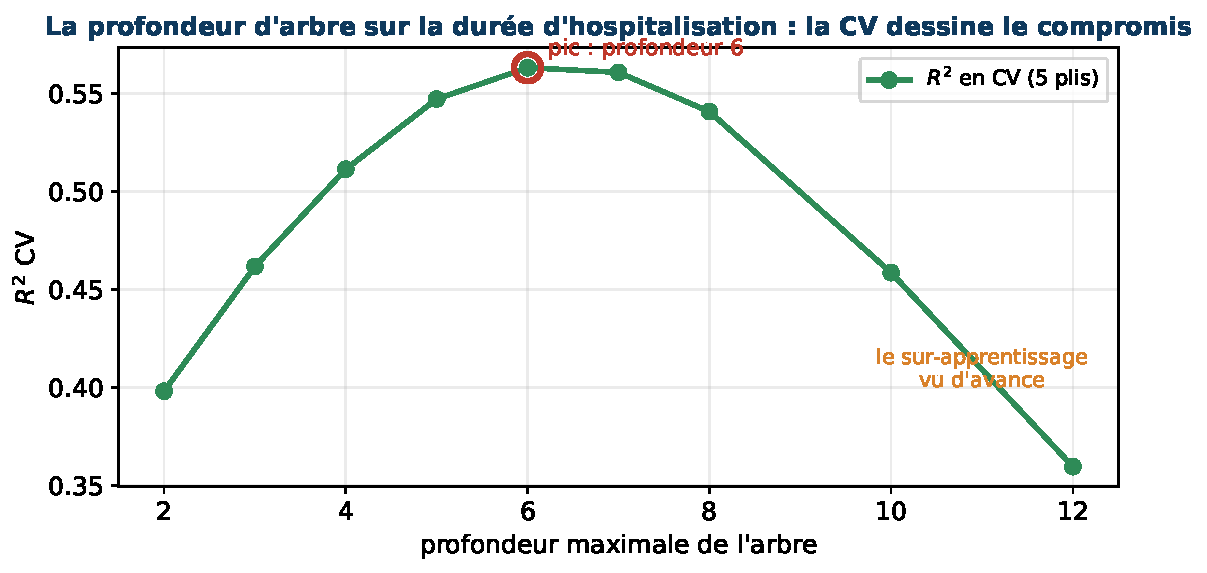
\includegraphics[width=0.60\linewidth]{f7_tree_cv}
\vspace{-2pt}

{\small Sur la durée d'hospitalisation : le $R^2$ de CV monte jusqu'à la profondeur $\mathbf{6}$ ($0{,}563$), plafonne, puis \emph{s'effondre} ($0{,}36$ à $12$). La Séance 5 avait montré le sur-apprentissage de la profondeur $10$ \emph{après coup}, sur le test ($0{,}726$ train contre $0{,}461$ test) ; la CV le voit \textbf{à l'avance}, sans dépenser le test.}
\end{frame}

\begin{frame}{Le protocole de réglage en trois temps}
\begin{ucadret}[Régler proprement, toujours pareil]
{\small \textbf{1.} Choisir les valeurs candidates et la métrique (Séance 6) $\to$ \textbf{2.} noter chaque candidate par CV \emph{sur l'entraînement seul} et garder la mieux notée $\to$ \textbf{3.} réentraîner la recette gagnante sur \emph{tout} l'entraînement, et seulement alors, verdict unique sur le test.}
\end{ucadret}
{\small Le score CV de la gagnante et son score test final diffèrent en général légèrement — c'est normal (le premier est un réglage gagnant parmi d'autres, donc un peu optimiste ; le second est la vérité). L'écart Ridge : CV $0{,}42$, test $0{,}336$ ; l'écart arbre : CV $0{,}569$, test $0{,}554$.}
\end{frame}

\begin{frame}{Exercice — lire une courbe de validation}
\begin{ucadrec}[Énoncé]
{\small Une courbe de validation donne, pour un hyperparamètre de complexité croissante, les scores CV $(0{,}41;\ 0{,}52;\ 0{,}58;\ 0{,}57;\ 0{,}44)$ pour les valeurs $(1, 2, 3, 4, 5)$. Identifier la valeur à retenir, la zone de sous-ajustement et la zone de sur-ajustement.}
\end{ucadrec}
\pause
\begin{ucadex}[Correction]
{\small Valeur retenue : $\mathbf{3}$ (pic à $0{,}58$ ; la valeur $4$, quasi équivalente à $0{,}57$, serait défendable — à bruit égal, préférer la plus \emph{simple}). Sous-ajustement : valeurs $1$–$2$, le modèle manque de capacité. Sur-ajustement : valeur $5$, la chute de $0{,}57$ à $0{,}44$ signe un modèle qui apprend le bruit — le même U que la Séance 5, mesuré sans toucher au test.}
\end{ucadex}
\end{frame}

% #####################################################################
\section{GridSearchCV : la grille}

\begin{frame}{L'idée : plusieurs curseurs à la fois}
\begin{ucaddef}[L'idée en une phrase]
{\small Quand deux hyperparamètres interagissent (la profondeur \emph{et} la taille minimale des feuilles d'un arbre), on note par CV \textbf{chaque combinaison} du produit cartésien — la \textbf{grille} — et on garde la meilleure case.}
\end{ucaddef}
{\small Les régler l'un après l'autre serait hasardeux : le meilleur réglage de l'un dépend souvent de la valeur de l'autre. La grille teste tout, au prix d'un coût qui se compte avant de lancer.}
\end{frame}

\begin{frame}{Le mécanisme — la double boucle}
\begin{ucadex}[GridSearchCV refait à la main, une case]
{\small La grille arbre sur la durée d'hospitalisation : \texttt{max\_depth} $\in \{3, 5, 7, 9\}$ $\times$ \texttt{min\_samples\_leaf} $\in \{1, 20, 100\}$, soit $12$ cases. Pour \emph{chaque} case, une CV complète à $5$ plis. La case $(5, 20)$, déroulée à la main :
\[ \text{scores des 5 plis} = (0{,}549;\ 0{,}532;\ 0{,}519;\ 0{,}579;\ 0{,}554) \;\Rightarrow\; \text{moyenne} = \mathbf{0{,}547} \]
C'est exactement le \texttt{mean\_test\_score} que \texttt{GridSearchCV} inscrit dans cette case. Tout l'outil tient en deux boucles : \emph{pour chaque combinaison, pour chaque pli} — entraîner, noter, moyenner.}
\end{ucadex}
\end{frame}

\begin{frame}{La grille en chiffres}
\centering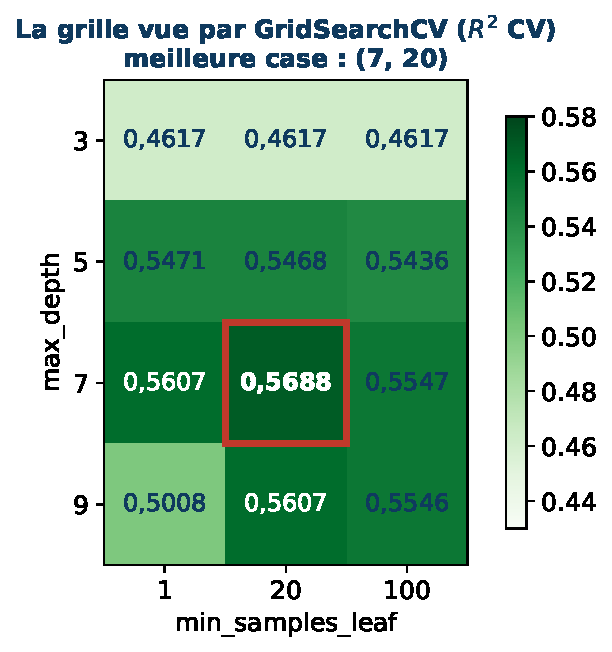
\includegraphics[width=0.34\linewidth]{f7_grid}
\vspace{-2pt}

{\small Meilleure case : \texttt{max\_depth} $= 7$, \texttt{min\_samples\_leaf} $= 20$, $R^2$ CV $= \mathbf{0{,}569}$. L'interaction se lit dans la colonne $9$ : la profondeur $9$ n'est bonne \emph{que} si les feuilles sont contraintes ($0{,}501$ seule, $0{,}561$ avec $20$) — régler les deux séparément aurait pu la manquer.}
\end{frame}

\begin{frame}[fragile]{En pratique : GridSearchCV}
\begin{lstlisting}
from sklearn.model_selection import GridSearchCV

grille = {"max_depth": [3, 5, 7, 9], "min_samples_leaf": [1, 20, 100]}
gs = GridSearchCV(DecisionTreeRegressor(random_state=0),
                  grille, cv=5, scoring="r2")
gs.fit(X_train, y_train)        # 12 combinaisons x 5 plis = 60 entrainements
print(gs.best_params_)          # {'max_depth': 7, 'min_samples_leaf': 20}
print(gs.best_score_)           # 0.569 (R2 de CV de la meilleure case)
print(gs.score(X_test, y_test)) # 0.554 : le verdict, une seule fois
\end{lstlisting}
{\small Après \texttt{fit}, l'objet a déjà \textbf{réentraîné} la recette gagnante sur tout l'entraînement (\texttt{refit=True} par défaut) : \texttt{gs} s'utilise directement comme modèle final. Pour une grille sur un Pipeline, préfixer le nom de l'étape : \texttt{"logisticregression\_\_C"}.}
\end{frame}

\begin{frame}{Le coût se compte avant de lancer}
\ucadformula{\text{nombre d'entraînements} \;=\; |\text{grille}| \times k \;+\; 1 \quad\text{(le refit final)}}
{\small La grille arbre : $12 \times 5 + 1 = \mathbf{61}$ entraînements. Une grille de trois hyperparamètres à dix valeurs chacun en CV $10$ plis : $10^3 \times 10 = 10\,001$ — souvent rédhibitoire. Réflexes d'économie : commencer par des grilles \emph{grossières} puis resserrer autour du gagnant ; et garder $k = 5$.}
\end{frame}

\begin{frame}{Exercice — budgéter une grille}
\begin{ucadrec}[Énoncé]
{\small Une grille croise $4$ valeurs de \texttt{C}, $2$ valeurs de \texttt{class\_weight} et $5$ valeurs de seuil, en CV stratifiée à $5$ plis. Compter les combinaisons puis le nombre total d'entraînements (refit compris). Un entraînement prend $2$ secondes : la recherche est-elle raisonnable ?}
\end{ucadrec}
\pause
\begin{ucadex}[Correction]
{\small Combinaisons : $4 \times 2 \times 5 = \mathbf{40}$. Entraînements : $40 \times 5 + 1 = \mathbf{201}$, soit environ $400$ secondes — moins de $7$ minutes : raisonnable. (Remarque d'expert : le seuil s'applique \emph{après} l'entraînement — les $5$ valeurs de seuil peuvent en réalité réutiliser les mêmes modèles, ramenant le vrai coût à $8 \times 5 + 1 = 41$ entraînements. Compter le coût, c'est aussi repérer ces économies.)}
\end{ucadex}
\end{frame}

% #####################################################################
\section{Le seuil, réglé proprement}

\begin{frame}{Le fil laissé par la Séance 6}
\begin{ucaddef}[L'idée en une phrase]
{\small Le seuil se règle sur des probabilités que le modèle n'a pas apprises par cœur. \texttt{cross\_val\_predict} fournit exactement cela : pour chaque patient de l'entraînement, la probabilité prédite \emph{par le tour de CV qui ne l'a pas vu} — des probabilités honnêtes, sur tout l'entraînement, sans toucher au test.}
\end{ucaddef}
{\small Différence avec \texttt{cross\_val\_score} : celui-ci rend $k$ \emph{notes} ; \texttt{cross\_val\_predict} rend $n$ \emph{prédictions} (une par observation, chacune venant du tour qui l'excluait). C'est la matière première idéale pour balayer un seuil.}
\end{frame}

\begin{frame}{Exemple — le seuil du paludisme par CV}
\begin{ucadex}[La mission de la Séance 6, protocole complet]
{\small Mission : recall $\geq 0{,}75$ avec la meilleure precision. \textbf{1.} Probabilités CV sur les $8\,000$ patients d'entraînement (\texttt{cross\_val\_predict}, $5$ plis stratifiés). \textbf{2.} Balayage des seuils sur ces probabilités : le gagnant est $s = \mathbf{0{,}125}$ (precision CV $0{,}200$, recall CV $0{,}751$). \textbf{3.} Réentraînement sur tout l'entraînement, puis verdict unique sur le test :
\[ \text{precision} = 0{,}205 \qquad \text{recall} = \mathbf{0{,}796} \]
Le seuil a tenu sa promesse sur des données jamais vues — et le test n'a servi qu'à la toute fin, une fois.}
\end{ucadex}
\end{frame}

\begin{frame}{La courbe du réglage honnête}
\centering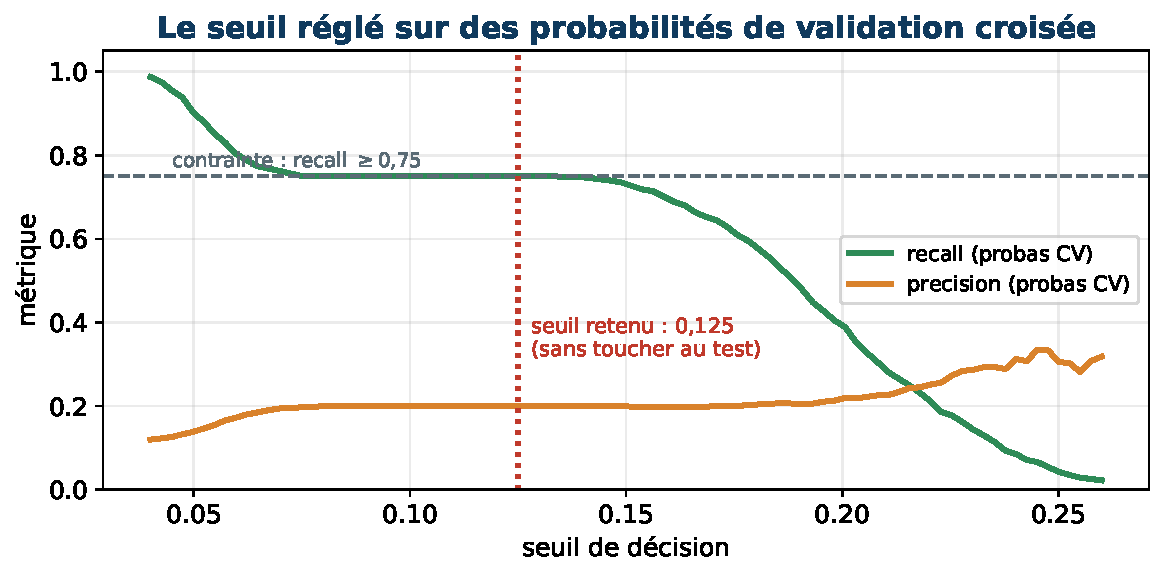
\includegraphics[width=0.66\linewidth]{f7_seuil_cv}
\vspace{-2pt}

{\small Le même graphique qu'en Séance 6 — mais tracé sur les probabilités de \emph{validation croisée}, pas sur le test. La différence est invisible à l'œil et fondamentale en principe : ce balayage-ci avait le droit d'exister \emph{avant} le verdict.}
\end{frame}

\begin{frame}{Exercice — trois protocoles, un seul honnête}
\begin{ucadrec}[Énoncé]
{\small Trois équipes règlent le seuil du même modèle. A : balaye les seuils sur le test, annonce le meilleur. B : balaye sur une tranche de validation unique, vérifie sur le test. C : balaye sur les probabilités de \texttt{cross\_val\_predict}, vérifie sur le test. Classer les trois protocoles du moins fiable au plus fiable, en justifiant.}
\end{ucadrec}
\pause
\begin{ucadex}[Correction]
{\small \textbf{A} : invalide — le chiffre annoncé est optimiste par construction (fuite, Séance 6). \textbf{B} : valide mais fragile — le seuil dépend du hasard d'\emph{une} tranche (la variance du début de séance). \textbf{C} : le plus fiable — le balayage s'appuie sur $n$ prédictions honnêtes couvrant tout l'entraînement, et le test reste un verdict vierge. Ordre : A $<$ B $<$ C.}
\end{ucadex}
\end{frame}

% #####################################################################
\section{Les pièges}

\begin{frame}{Piège — standardiser avant de découper}
\begin{ucadpiege}[La fuite qui se glisse dans la CV]
{\small Standardiser \emph{tout} l'entraînement \textbf{puis} lancer la CV est une fuite : la moyenne et l'écart-type utilisés dans chaque tour ont vu les données du pli de validation — le juge a reçu une confidence. La parade est déjà connue : passer le \textbf{Pipeline entier} à la CV, qui refait \texttt{StandardScaler} \emph{à l'intérieur} de chaque tour, sur le seul entraînement du tour.}
\end{ucadpiege}
{\small C'est la règle de la Séance 4 — « le préprocesseur s'ajuste sur le train seul » — appliquée récursivement : \emph{chaque tour de CV a son propre train}. Tout ce qui apprend des données (imputation, standardisation, encodage) doit vivre dans le Pipeline, jamais avant.}
\end{frame}

\begin{frame}{Piège — la grille optimiste}
\begin{ucadpiege}[Le gagnant a aussi eu de la chance]
{\small \texttt{best\_score\_} est le maximum de $12$ (ou $200$) moyennes bruitées : le gagnant gagne en partie par mérite, en partie par chance — son score CV est donc légèrement \textbf{optimiste}, et l'optimisme grandit avec la taille de la grille. C'est précisément pour cela que le verdict final se prend sur le test, jamais sur \texttt{best\_score\_}.}
\end{ucadpiege}
{\small Les chiffres du jour l'illustrent sans drame : grille arbre, CV $0{,}569$ contre test $0{,}554$ ; Ridge, CV $0{,}42$ contre test $0{,}336$ (ici l'écart joue dans l'autre sens — le bruit va dans les deux directions, l'optimisme n'est qu'une \emph{tendance}).}
\end{frame}

\begin{frame}{Piège — le test consulté « juste pour voir »}
\begin{ucadpiege}[Chaque consultation dépense le test]
{\small Regarder le test après chaque essai, « pour information », puis continuer à régler, recrée la fuite en silence : les choix suivants sont influencés par ce qui a été vu. Discipline du cours : le test est \textbf{scellé} pendant tout le développement ; une seule ouverture, à la fin, et le chiffre obtenu est définitif — bon ou mauvais.}
\end{ucadpiege}
{\small Si le verdict final déçoit, la tentation est de « réessayer un peu » puis de re-tester : à ce moment le test est devenu une validation, et il faudrait de nouvelles données pour juger. Mieux vaut prévenir : ne desceller qu'une fois sûr.}
\end{frame}

% #####################################################################
\section{Synthèse}

\begin{frame}{Le bilan : tous les réglages du cours, un seul protocole}
\begin{ucadex}[Ce que la séance a réglé, chiffres en main]
{\small \begin{center}\footnotesize\renewcommand{\arraystretch}{1.12}\begin{tabular}{l|l|l|l}
réglage & méthode & choix par CV & verdict test\\\hline
$\alpha$ de Ridge (sinusoïde S5) & courbe de validation & $\alpha = 0{,}1$ & RMSE $0{,}336$\\
profondeur d'arbre (durée) & courbe de validation & $6$ & —\\
arbre : profondeur $\times$ feuilles & GridSearchCV & $(7, 20)$ & $R^2$ $0{,}554$\\
seuil de la logistique (palu) & cross\_val\_predict & $0{,}125$ & recall $0{,}796$\\
\end{tabular}\end{center}
Quatre réglages, quatre outils — un seul principe : noter par CV sur l'entraînement, geler, juger une fois.}
\end{ucadex}
\end{frame}

\begin{frame}{Le protocole complet, de bout en bout}
\begin{ucadret}[Le rituel à dérouler sur tout nouveau problème]
{\small \textbf{1.} Split stratifié train/test, le test au coffre $\to$ \textbf{2.} baseline (Séances 3 et 6) $\to$ \textbf{3.} la recette dans un \textbf{Pipeline} (préprocesseurs compris) $\to$ \textbf{4.} CV stratifiée à $5$ plis pour estimer, courbes de validation ou \textbf{GridSearchCV} pour régler, \texttt{cross\_val\_predict} pour le seuil $\to$ \textbf{5.} réentraîner la recette gagnante sur tout le train $\to$ \textbf{6.} ouvrir le test, une fois : métriques alignées sur la mission (Séance 6), chiffre définitif.}
\end{ucadret}
\end{frame}

\begin{frame}{À retenir — Séance 7}
\begin{ucadret}[L'essentiel]
\begin{itemize}\small
  \item Trois usages, trois jeux : ce qui \textbf{règle} ne peut plus \textbf{juger} ; le test ne sert qu'une fois.
  \item Un score sur un split unique est une mesure \textbf{bruitée} (étendue $0{,}016$ sur le paludisme) — comparer des recettes exige des moyennes.
  \item La \textbf{CV à $k$ plis} : $k$ entraînements, chaque donnée juge une fois, verdict $=$ moyenne $\pm$ écart-type ; elle évalue une \emph{recette}, le modèle final se réentraîne sur tout.
  \item Classification $\Rightarrow$ \textbf{plis stratifiés} ; $k = 5$ par défaut.
  \item \textbf{Courbe de validation} pour un curseur, \textbf{GridSearchCV} pour plusieurs (coût $= |\text{grille}| \times k + 1$), \textbf{cross\_val\_predict} pour le seuil.
  \item Le Pipeline entre \emph{dans} la CV — standardiser avant les plis est une fuite ; \texttt{best\_score\_} est optimiste — le test tranche.
\end{itemize}
\end{ucadret}
\end{frame}

\begin{frame}{Pièges fréquents}
\begin{itemize}\small
  \item Régler un hyperparamètre (ou un seuil) sur le test — la fuite originelle.
  \item Standardiser ou imputer \emph{avant} la CV au lieu de l'inclure dans le Pipeline.
  \item Oublier la stratification sur une classe rare : des plis qui jugent des problèmes différents.
  \item Croire que la CV produit un modèle — elle note une recette ; le modèle final se réentraîne.
  \item Prendre \texttt{best\_score\_} pour le niveau réel : c'est un maximum de mesures bruitées, donc optimiste.
  \item Surinterpréter les petites bosses d'une courbe de validation bruitée (les $30$ points de Ridge).
  \item Lancer une grille sans compter ses entraînements.
  \item Rouvrir le test « juste pour voir » après un premier verdict.
\end{itemize}
\end{frame}

\begin{frame}{Prochaine séance}
\begin{ucadfront}[Séance 8 — La force du nombre : les méthodes d'ensemble]
{\small Le mini-défi du TP règle un arbre sur le paludisme par CV : bien réglé, il rivalise avec la logistique — puis plafonne. La Séance 8 dépasse ce plafond par une idée simple et puissante : entraîner \emph{beaucoup} d'arbres et les faire voter — les forêts aléatoires, puis le boosting.}
\end{ucadfront}
\end{frame}

\begin{frame}{Références}
\begin{itemize}\small
  \item James, Witten, Hastie, Tibshirani — \emph{An Introduction to Statistical Learning}, 2\textsuperscript{e} éd., Springer, 2021.
  \item Géron — \emph{Hands-On Machine Learning}, 3\textsuperscript{e} éd., O'Reilly, 2022.
  \item Müller, Guido — \emph{Introduction to Machine Learning with Python}, O'Reilly, 2016.
  \item Cours : University of Washington CSE 446 ; Stanford CS229.
\end{itemize}
\end{frame}

\end{document}
